\documentclass[11pt]{article}
\usepackage[margin=1in]{geometry}
\usepackage{amsmath,amssymb,amsthm}
\usepackage{tikz}
\usepackage[colorlinks=true,linkcolor=blue,citecolor=blue,urlcolor=blue,pdfauthor={P. Graham}]{hyperref}
\newtheorem{theorem}{Theorem}
\newtheorem{lemma}[theorem]{Lemma}
\DeclareMathOperator{\opx}{opx}
\newcommand{\R}{\mathbb R}
\newcommand{\area}{\lambda}
\title{A proof of Geneson's continuous gluing conjecture}
\author{P. Graham\\ \small\url{https://orcid.org/0009-0007-8493-1505}}
\date{November 2, 2026}
\begin{document}
\maketitle
\begin{abstract}
Geneson introduced continuous Tur\'an numbers: for a set $R\subseteq\R^2$ and $n>0$, $\opx(n,R)$ is the supremum of the areas of open subsets of the square $[0,n]^2$ that contain no copy of $R$, where a copy may move the horizontal coordinates of $R$ apart and its vertical coordinates apart, keeping their order, but never closer together. We prove Conjecture 6.3 of Geneson's \emph{Continuous Tur\'an numbers}: if $P$ and $Q$ share a point $(c,d)$, with $P$ weakly south-west of it and $Q$ weakly north-east of it, then $\opx(n,P\cup Q)\le\opx(n,P)+\opx(n,Q)$ for every $n>0$. The sets $P$ and $Q$ are arbitrary: no finiteness, boundedness or measurability is assumed. Keszegh proved the corresponding inequality for forbidden zero--one matrices joined at opposite corner entries, by partitioning a host matrix according to the possible gluing corners. We carry this partition over to the continuous setting. What we add is compactness of the space of copies in a compact host, which makes the partition measurable, and the inner regularity of Lebesgue measure, which passes from measurable pieces to open sets. The theorem and its proof are formalized in Lean.

This work has not yet been reviewed by experts. The proofs, the Lean formalization and the text were produced by AI models (from OpenAI and Anthropic), working under the author's direction.
\end{abstract}
\medskip
\noindent\textit{2020 Mathematics Subject Classification:} 05D99, 28A75.\\
\textit{Keywords:} continuous Tur\'an numbers, forbidden patterns, gluing, compactness.

\section{Introduction}
Geneson introduced continuous Tur\'an numbers as an area analogue of extremal functions for forbidden zero--one matrices \cite{Geneson}. A pattern is any subset $R$ of the plane. A set $S$ contains $R$ if $S$ holds a copy of $R$ obtained by moving the $x$-coordinates of $R$ apart and its $y$-coordinates apart, never closer, while keeping their order; the exact definition follows. Geneson observes that ``for a better understanding of $\opx(n,P)$, it would be useful to find more operations'', recalls Keszegh's gluing theorem for zero--one matrices, and asks: ``Is an analogous operation possible for subsets of $\R^2$?'' \cite[p.~32]{Geneson}. Conjecture 6.3 of \cite{Geneson} is the corresponding inequality for patterns joined at opposite corners. We prove it as stated there: $P$ and $Q$ may be arbitrary subsets of the plane, with no finiteness, boundedness or measurability assumed.

Write $X_R=\{x:\exists y,\ (x,y)\in R\}$ and $Y_R=\{y:\exists x,\ (x,y)\in R\}$ for the coordinate projections of $R\subseteq\R^2$. Following the definition on page 2 of \cite{Geneson}, a set $S$ \emph{contains} $R$ if there are maps
\[
 f:X_R\longrightarrow X_S,\qquad g:Y_R\longrightarrow Y_S
\]
such that $(f(x),g(y))\in S$ whenever $(x,y)\in R$, and
\begin{equation}\label{eq:expand}
 f(x')-f(x)\ge x'-x\quad(x<x'),\qquad
 g(y')-g(y)\ge y'-y\quad(y<y').
\end{equation}
(The journal version states these inequalities in this difference form; arXiv v1 writes them as ratios at least one, which is equivalent since the denominators are positive.) The maps are defined only on the coordinate projections. They need not extend to maps on all of $\R$. A set \emph{avoids} $R$ when it does not contain $R$.

For $n>0$ put $B_n=[0,n]^2$ and $U_n=(0,n)^2$, and let $\area$ denote planar Lebesgue measure. For a nonempty pattern $R$, define, in Geneson's notation,
\begin{equation}\label{eq:opx}
 \opx(n,R)=\sup\{\area(S):S\subseteq B_n,\ S\text{ open in }\R^2,\ S\text{ avoids }R\}.
\end{equation}
Here we read ``open'' as open in $\R^2$, not just relatively open in $B_n$; this is the reading formalized in Lean (Section~\ref{sec:verify}).

\begin{theorem}\label{thm:main}
Let $n>0$, let $P,Q\subseteq\R^2$, and let $c,d\in\R$. Suppose that $(c,d)\in P\cap Q$ and
\[
 P\subseteq(-\infty,c]\times(-\infty,d],\qquad
 Q\subseteq[c,\infty)\times[d,\infty).
\]
Then
\[
 \opx(n,P\cup Q)\le \opx(n,P)+\opx(n,Q).
\]
\end{theorem}

We call $(c,d)$ the \emph{anchor}: every point of $P$ lies weakly south-west of it and every point of $Q$ weakly north-east of it.

\begin{figure}[ht]
\centering
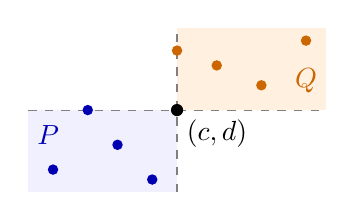
\begin{tikzpicture}[scale=.63]
\fill[blue!6] (-3,-1.65) rectangle (0,0);
\fill[orange!12] (0,0) rectangle (3,1.65);
\draw[dashed,gray] (-3,0)--(3,0); \draw[dashed,gray] (0,-1.65)--(0,1.65);
\foreach \x/\y in {-2.5/-1.2,-1.2/-.7,-.5/-1.4,-1.8/0} \fill[blue!70!black] (\x,\y) circle(3pt);
\foreach \x/\y in {.8/.9,1.7/.5,2.6/1.4,0/1.2} \fill[orange!80!black] (\x,\y) circle(3pt);
\fill (0,0) circle(3.5pt);\node[below right] at (0,0){$(c,d)$};
\node[blue!70!black] at (-2.6,-.5){$P$};\node[orange!80!black] at (2.6,.6){$Q$};
\end{tikzpicture}
\caption{The common anchor and the two allowed quadrants. Points on the boundary lines are allowed; the theorem is not restricted to finite patterns.}
\end{figure}

Keszegh's finite gluing theorem (2009, Theorem 2.2 in \cite{Keszegh}) is the predecessor of Theorem~\ref{thm:main}: if matrices with a bottom-right and a top-left one are joined at those entries, the extremal function of the joined matrix is at most the sum of the separate extremal functions. (Reading the column index as $x$ and the row index, which increases downward, as $y$, this is the configuration of Theorem~\ref{thm:main}.) We use that theorem's partition idea, while proving the required continuous version directly. Geneson's Theorem 3.1 in the journal version of \cite{Geneson} gives a $\Theta$ comparison with the matrix extremal function for finite planar patterns. That comparison does not give the exact inequality of Theorem~\ref{thm:main}, with constant one, for arbitrary planar sets.

The proof has two analytic tasks. First, the set of possible gluing corners in a compact host must be measurable. Second, an avoiding measurable piece must have area at most the supremum over \emph{open} avoiding sets. Compact spaces of coordinate maps resolve both tasks. The remaining argument is the corner partition and inner regularity of Lebesgue measure.

Two related works concern finite objects: forcing patterns in $(0,1)$-matrices \cite{CaoTsai}, and intersections and circuits in finite sets of line segments \cite{Brimkov,BrimkovArXiv}. Neither treats the area of open sets avoiding a planar pattern.

\section{Compact witnesses and gluing}
A \emph{witness} for a copy of $R$ in $K$ is a pair of real-valued maps on $X_R,Y_R$ satisfying \eqref{eq:expand}, with every image point in $K$. Since each $(f(x),g(y))$ lies in $K$, $f$ takes values in $X_K$ and $g$ in $Y_K$, so witnesses are exactly the pairs of maps in the definition of containment.

\begin{lemma}\label{lem:compact}
For compact $K\subseteq B_n$, the space of witnesses for $R$ in $K$ is compact in the topology of pointwise convergence. For $a\in R$, the set of images of $a$ under these witnesses is compact.
\end{lemma}
\begin{proof}
Every coordinate of $R$ occurs in some point of $R$. Thus every value of a witness into $K$ lies in $[0,n]$. Work in the compact product
\[
 \mathcal W_R=[0,n]^{X_R}\times[0,n]^{Y_R},
\]
whose compactness follows from the product theorem, with no restriction on the index sets. For fixed $x<x'$, the condition $f(x')-f(x)\ge x'-x$ is closed, since coordinate evaluations and subtraction are continuous. The same holds for the vertical inequalities. For each $(x,y)\in R$, the condition $(f(x),g(y))\in K$ is closed because $K$ is closed. The witness space is the intersection of all these closed conditions, hence is compact. The map sending a witness to the image of $a$ is continuous, so the set of these images is compact as well.
\end{proof}

\begin{lemma}\label{lem:glue}
Under the quadrant hypotheses of Theorem~\ref{thm:main}, copies of $P$ and $Q$ in the same host with the same image of $(c,d)$ combine to a copy of $P\cup Q$.
\end{lemma}
\begin{proof}
Write $f_P,f_Q$ for the horizontal maps. Their domains lie respectively to the left and right of $c$, so the domains intersect only at $c$. The maps agree there. They therefore define a map on $X_P\cup X_Q$. The expansion inequalities within either domain are unchanged. For $x\in X_P$ and $x'\in X_Q$,
\[
 f_Q(x')-f_P(x)
 =[f_Q(x')-f_Q(c)]+[f_P(c)-f_P(x)]
 \ge (x'-c)+(c-x)=x'-x.
\]
Since $X_P\subseteq(-\infty,c]$ and $X_Q\subseteq[c,\infty)$, a pair $x<x'$ that does not lie in a single domain has $x\in X_P$ and $x'\in X_Q$, so the displayed case is the only mixed one. The vertical maps combine in the same way at $d$. Each image point is one of the original image points, so belongs to the host.
\end{proof}

\begin{lemma}\label{lem:partition}
Under the hypotheses of Theorem~\ref{thm:main}, suppose $K\subseteq B_n$ is compact and avoids $P\cup Q$. Let $A$ be the set of images of $(c,d)$ under copies of $P$ in $K$. Then $A$ is a compact subset of $K$ avoiding $Q$, and $K\setminus A$ is measurable and avoids $P$.
\end{lemma}
\begin{proof}
Lemma~\ref{lem:compact} gives compactness, and the anchor belongs to $P$, so $A\subseteq K$. If $A$ contained $Q$, let $z$ be the image of the anchor in this copy. By the definition of $A$, there would be a copy of $P$ in $K$ anchored at $z$. Lemma~\ref{lem:glue} would produce a copy of $P\cup Q$ in $K$, a contradiction. If $K\setminus A$ contained $P$, the anchor of that copy would belong both to $A$ and to $K\setminus A$, also a contradiction. Finally, compact sets are closed, so $K\setminus A$ is Borel measurable.
\end{proof}

\section{From measurable pieces to open sets}
The next lemma ensures that the open-set supremum controls the measurable pieces in Lemma~\ref{lem:partition}.

\begin{lemma}\label{lem:collar}
If a compact set $C\subseteq U_n$ avoids a nonempty pattern $R$, there exists an ambient-open set $O$ with $C\subseteq O\subseteq B_n$ that avoids $R$.
\end{lemma}
\begin{proof}
If $C$ is empty, take $O=\varnothing$. Otherwise, for $\varepsilon>0$ put
\[
 K_\varepsilon=\{z\in B_n:\operatorname{dist}(z,C)\le\varepsilon\}.
\]
These are compact. If every $K_\varepsilon$ contained $R$, their witness spaces would be nonempty closed subsets of the single compact space $\mathcal W_R$ from Lemma~\ref{lem:compact}. They are nested as $\varepsilon$ decreases, so have the finite intersection property. A witness in their intersection maps every point of $R$ into $\bigcap_{\varepsilon>0}K_\varepsilon=C$, contradicting avoidance. Some $K_\varepsilon$ therefore avoids $R$. The open set
\[
 O=\{z\in U_n:\operatorname{dist}(z,C)<\varepsilon\}
\]
contains $C$ and is contained in $K_\varepsilon$, hence avoids $R$.
\end{proof}

\begin{lemma}\label{lem:transfer}
If $R$ is nonempty and $E\subseteq B_n$ is measurable and avoids $R$, then $\area(E)\le\opx(n,R)$.
\end{lemma}
\begin{proof}
The boundary $B_n\setminus U_n$ has measure zero. Hence $E\cap U_n$ has the same measure as $E$. Every compact $C\subseteq E\cap U_n$ avoids $R$. By Lemma~\ref{lem:collar}, it lies in an open avoiding set $O\subseteq B_n$, giving
\[
 \area(C)\le\area(O)\le\opx(n,R).
\]
Inner regularity of Lebesgue measure says that the measure of the measurable, finite-measure set $E\cap U_n$ is the supremum of the measures of its compact subsets. Taking that supremum proves the assertion.
\end{proof}

\begin{proof}[Proof of Theorem~\ref{thm:main}]
Let $S\subseteq B_n$ be open and avoid $P\cup Q$. For any compact $K\subseteq S$, apply Lemma~\ref{lem:partition}. The two disjoint measurable pieces $A$ and $K\setminus A$ avoid $Q$ and $P$, respectively. Both patterns are nonempty because they contain the anchor. Lemma~\ref{lem:transfer} and finite additivity give
\[
 \area(K)=\area(A)+\area(K\setminus A)
 \le\opx(n,Q)+\opx(n,P).
\]
Inner regularity gives the same bound for $\area(S)$. Finally, taking the supremum over all such open $S$ yields the required inequality. No measurability property of $P$ or $Q$ was used: only the host sets and their witness spaces needed topological or measure properties.
\end{proof}

\section{Verification and reproducibility}\label{sec:verify}
The Lean theorem \texttt{Geneson.geneson\_conjecture\_6\_3} has parameters $n\in\R$, $n>0$, arbitrary $P,Q:\mathrm{Set}(\R\times\R)$ and $c,d\in\R$, followed by exactly the two anchor-membership and two quadrant hypotheses in Theorem~\ref{thm:main}. Its conclusion is the inequality for the supremum defined in \eqref{eq:opx}. The definition of area is the real value of Lebesgue measure; all sets used for this value are contained in the finite-measure square.

Its containment definition, \texttt{Geneson.Contains}, states the expansion conditions as ratios at least one, as in arXiv v1 of \cite{Geneson}.

The formalization proves the witness equivalence, compactness, gluing, open-neighborhood lemma and inner-regularity transfer. A second Lean theorem, \texttt{SrcCheck.conjecture\_6\_3\_source}, restates the definitions independently, with containment in the difference form \eqref{eq:expand} and with the quadrant conditions imposed only on points other than the anchor, as in Conjecture 6.3 of \cite{Geneson}. It is derived from the first theorem through proved equivalences; at the anchor the omitted conditions hold trivially, so this is the same statement.

The Lean files are in the folder \texttt{lean} that accompanies this paper. From that folder, run \texttt{lake exe cache get} and then \texttt{lake build}; the toolchain and dependencies are pinned there. The build also checks the theorem's statement and two small examples: a single point has $\opx$ zero, and an open vertical strip of width $c$ avoids a horizontal segment of length $c$. The proof uses only the standard Lean axioms of propositional extensionality, classical choice and quotient soundness, which the build checks. It relies on the Lean kernel and mathlib's topology, measure theory and real analysis; it does not rely on an external numerical computation.

\begin{thebibliography}{9}
\bibitem{Geneson}
Jesse Geneson, \emph{Continuous Tur\'an numbers}, Integers \textbf{24} (2024), A1.
\href{https://doi.org/10.5281/zenodo.10450893}{doi:10.5281/zenodo.10450893}.
Preprint \href{https://arxiv.org/abs/2105.04864v1}{arXiv:2105.04864v1}, May 11, 2021.
References to page numbers and Theorem 3.1 are to the journal version; Conjecture 6.3 appears in both versions.
\bibitem{Keszegh}
Bal\'azs Keszegh, \emph{On linear forbidden submatrices}, Journal of Combinatorial Theory, Series A \textbf{116} (2009), 232--241, Theorem 2.2.
\href{https://doi.org/10.1016/j.jcta.2008.05.006}{doi:10.1016/j.jcta.2008.05.006}.
\bibitem{CaoTsai}
Lei Cao and Shen-Fu Tsai, \emph{Pattern forcing $(0,1)$-matrices}, Linear Algebra and its Applications (2026).
\href{https://doi.org/10.1016/j.laa.2026.10.005}{doi:10.1016/j.laa.2026.10.005}.
Cited from the preprint \href{https://arxiv.org/abs/2510.27076v1}{arXiv:2510.27076v1}, October 31, 2025.
\bibitem{Brimkov}
Boris Brimkov, Jesse Geneson, Alathea Jensen, Jordan Broussard and Pouria Salehi Nowbandegani, \emph{Intersections and circuits in sets of line segments}, Journal of Combinatorial Optimization \textbf{44} (2022), 2302--2323.
\href{https://doi.org/10.1007/s10878-021-00731-3}{doi:10.1007/s10878-021-00731-3}.
\bibitem{BrimkovArXiv}
Boris Brimkov, Jesse Geneson, Alathea Jensen, Jordan Miller and Pouria Salehi Nowbandegani, \emph{Intersections, circuits, and colorability of line segments}, preprint of \cite{Brimkov}, \href{https://arxiv.org/abs/1808.07176v1}{arXiv:1808.07176v1}, August 22, 2018.
\end{thebibliography}
\end{document}
